\section{Sample \& Hold}
\subsection{Objetivo}
El objetivo principal de esta sección es analizar y comprender las no idealidades presentes en el circuito integrado Sample \& Hold  LF398 a través de simulaciones, evaluando su comportamiento bajo distintas condiciones de operación tomando como referencia las siguientes señales de entrada, con $fs = 10kHz$ y $A_{max} = 2.5V$:
\begin{itemize}
	\item $x_1(t) = A_{max} \cdot sin(2\pi \cdot fs/12 \cdot t)$
	\item $x_2(t) = A_{max} \cdot sin(2\pi \cdot fs/3 \cdot t)$
\end{itemize}
\subsection{Comparativa de Capacitores de Hold ($C_h$)}

Para evaluar el impacto del capacitor de hold en el rendimiento del circuito, se simularon dos casos extremos:

\subsubsection{Caso 1: $C_h \le 150pF$}
En este escenario se utiliza un capacitor de valor reducido. Como se observa en la Figura \ref{fig:ch_bajo}, el principal beneficio es una \textbf{alta velocidad de adquisición}, lo que permite rastrear variaciones rápidas de la señal. Sin embargo, esto trae una mayor susceptibilidad al ruido.

\begin{figure}[H]
	\begin{subfigure}{0.45\textwidth}
		\centering
		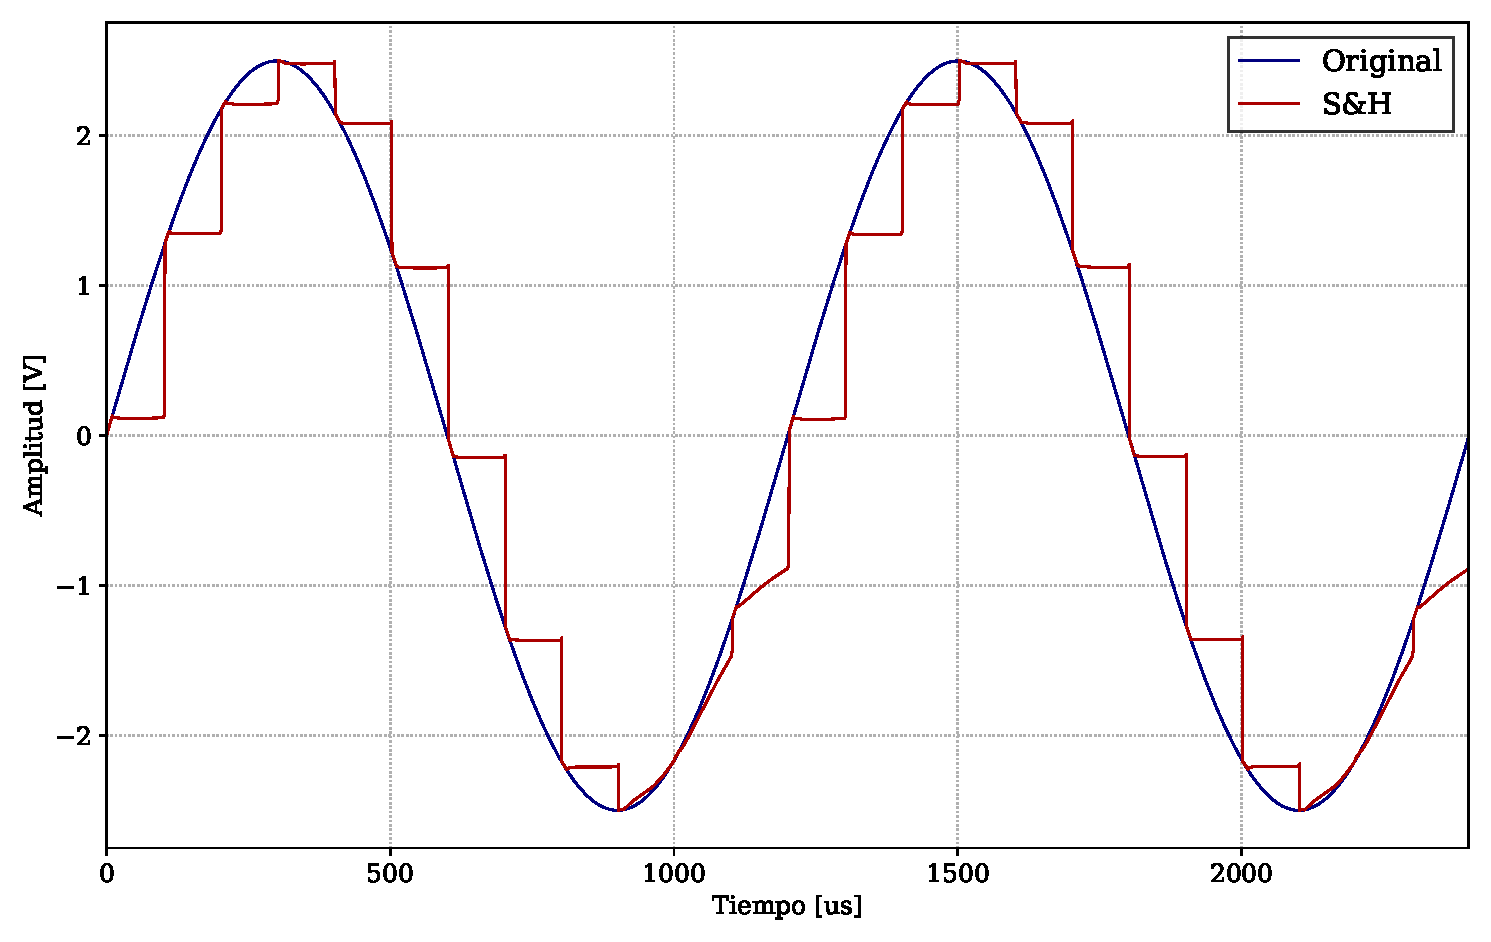
\includegraphics[width=\textwidth]{Imagenes/4_S&H/Ch_150p_833.pdf}
		\caption{Simulación con $C_h = $150pF a $f_s/12$.}
		\label{fig:ch_bajo}
	\end{subfigure}
	\hfill
	\begin{subfigure}{0.45\textwidth}
		\centering
		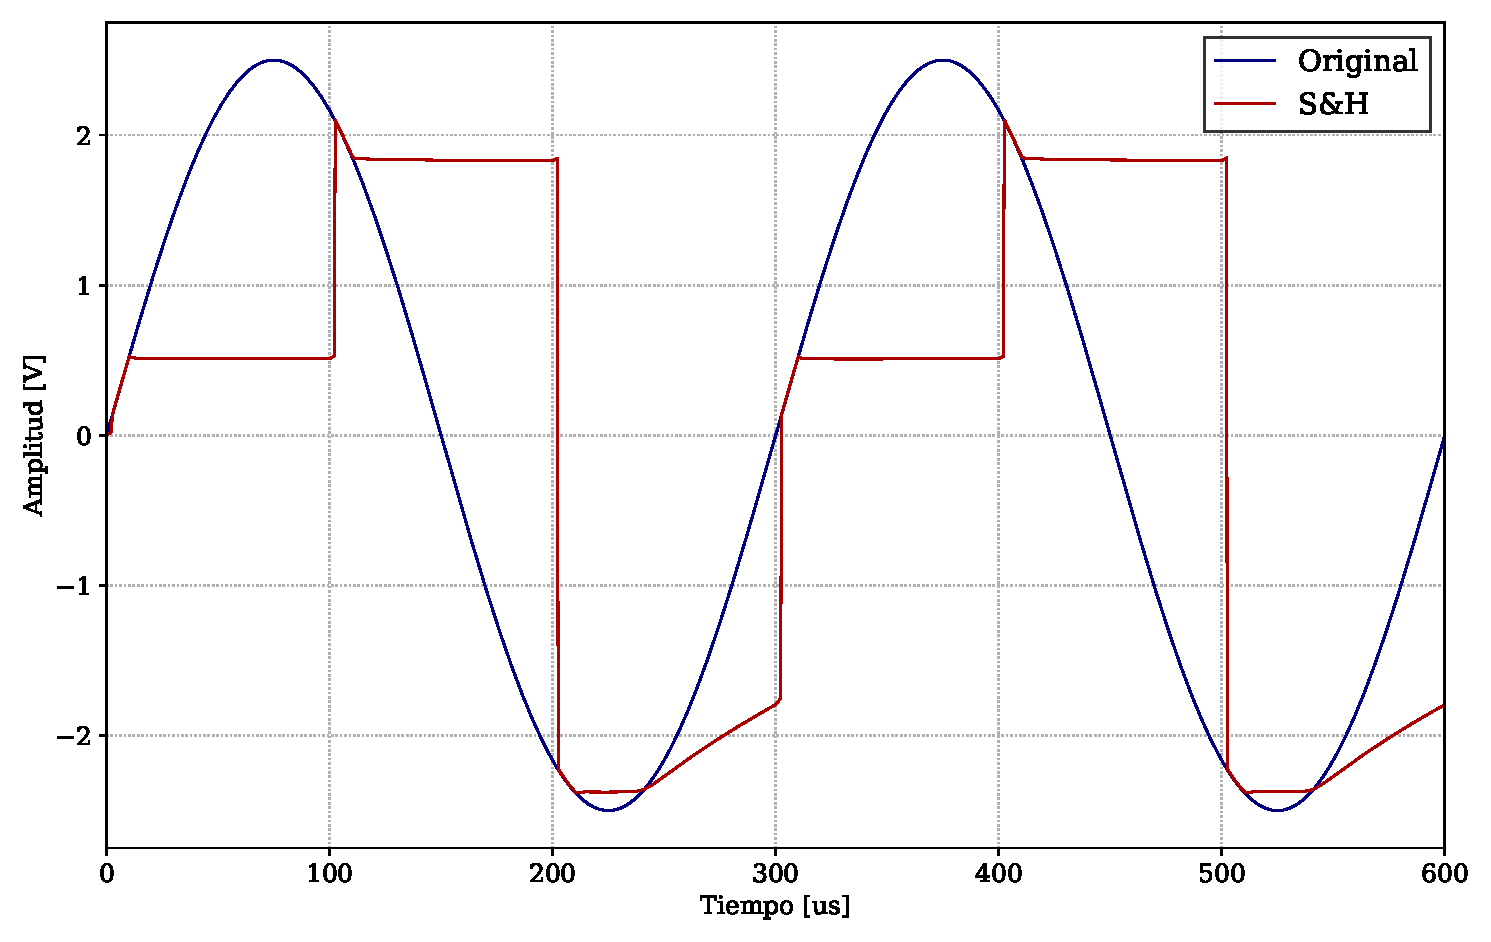
\includegraphics[width=\textwidth]{Imagenes/4_S&H/Ch_150p_3333.pdf}
		\caption{Simulación con $C_h = $150pF a $f_s/3$.}
		\label{fig:ch_bajo}
	\end{subfigure}
\end{figure}
\newpage
\subsubsection{Caso 2: $C_h \ge 47nF$}
Al incrementar el valor del capacitor, la señal retenida se vuelve mucho más estable en el tiempo durante el estado de hold. La desventaja de esta configuración, visible en la Figura \ref{fig:ch_bajo}, es el aumento significativo en el \textbf{tiempo de adquisición} ($acquisition \ time$), lo que limita la frecuencia máxima de la señal de entrada que el sistema puede muestrear correctamente. Generando un defesamiento y atenuación de potencia con respecto a la señal original.

\begin{figure}[H]
	\begin{subfigure}{0.45\textwidth}
		\centering
		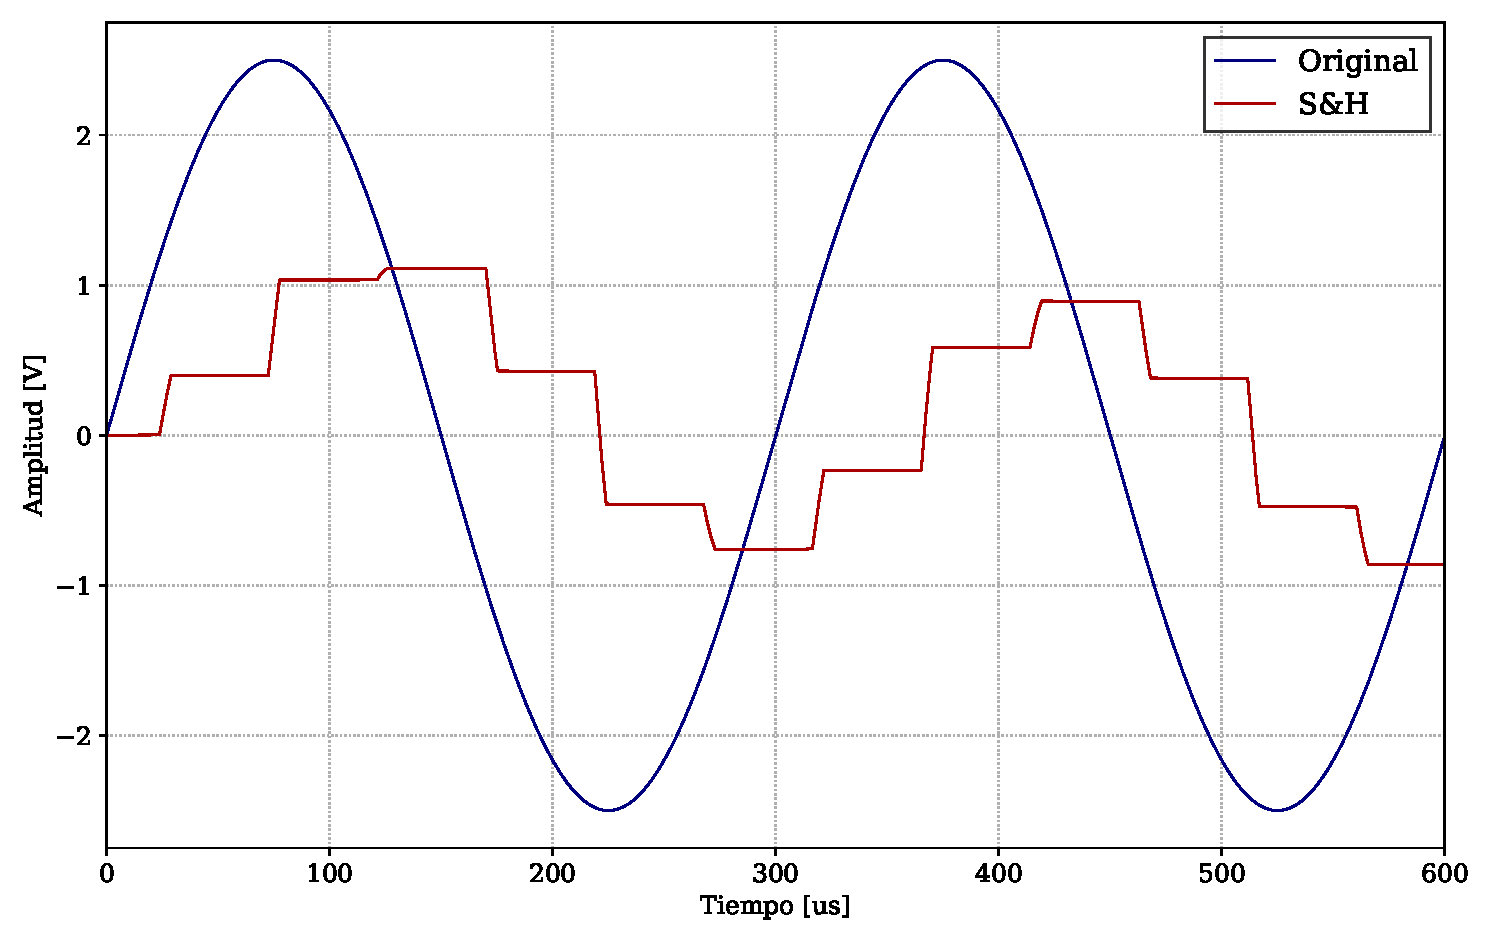
\includegraphics[width=\textwidth]{Imagenes/4_S&H/Ch_47n_833.pdf}
		\caption{Simulación con $C_h = 47$pF a $f_s/12$. Se observa el alto droop rate y la rápida adquisición.}
		\label{fig:ch_bajo}
	\end{subfigure}
	\hfill
	\begin{subfigure}{0.45\textwidth}
		\centering
		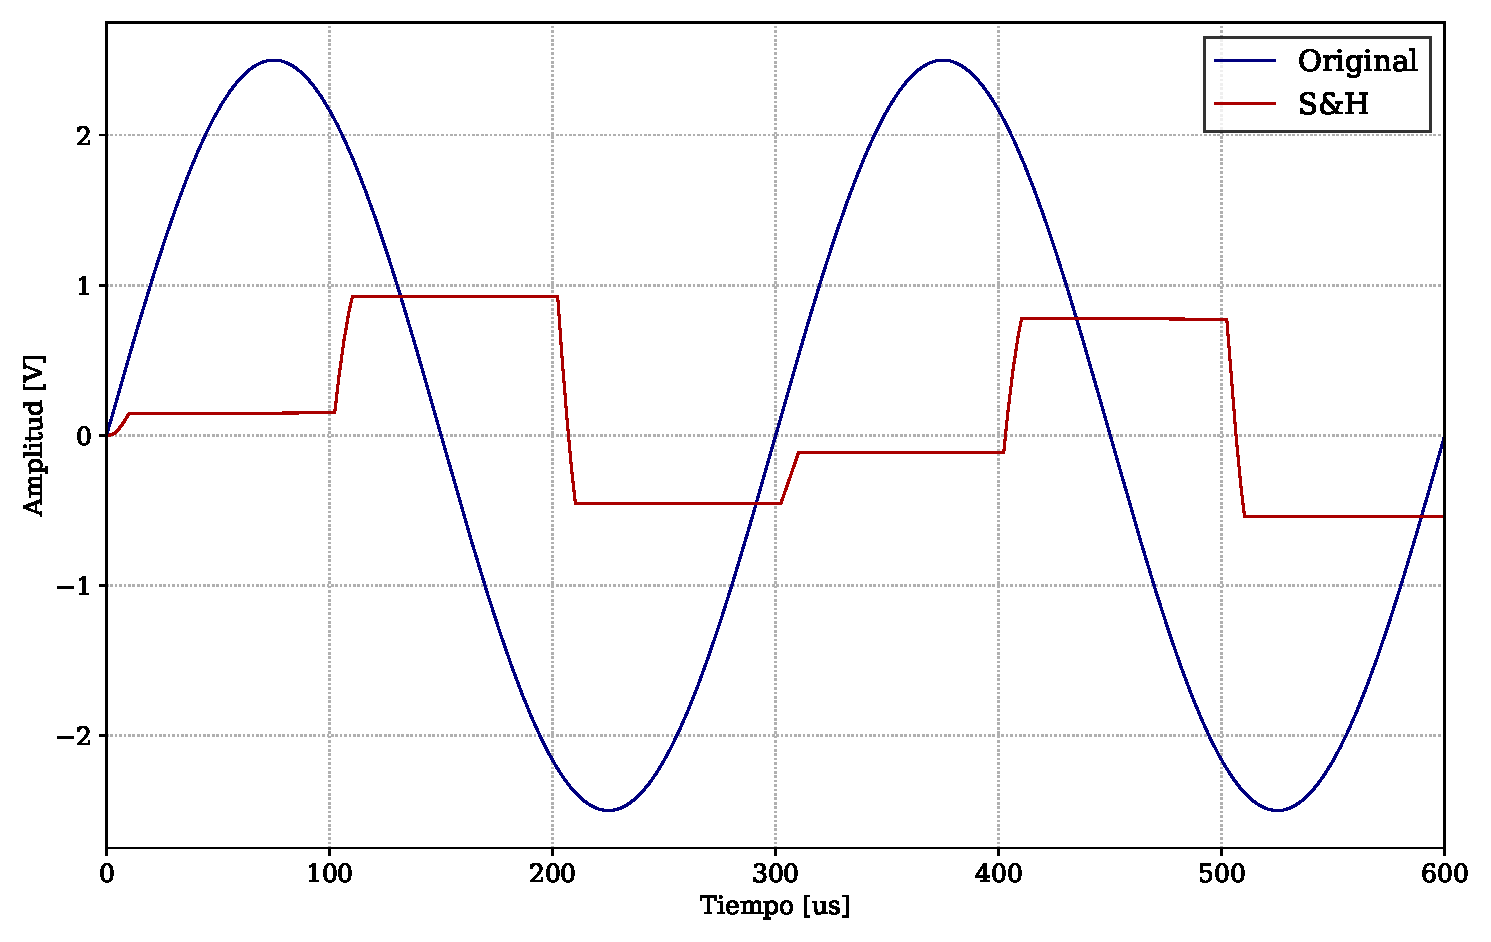
\includegraphics[width=\textwidth]{Imagenes/4_S&H/Ch_47n_3333.pdf}
		\caption{Simulación con $C_h = 47$pF a $f_s/3$. Se observa el alto droop rate y la rápida adquisición.}
		\label{fig:ch_bajo}
	\end{subfigure}
\end{figure}

\subsubsection{Conclusión respecto al capacitor hold}
De acuerdo a lo visto a las simulaciones, es que al reducir el valor de capacitancia se muestrea de mejor manera las señales de mayor frecuencia, sin embargo, puede llegar a generar inestabilidad en los picos negativos de la señal original.
Asimismo, se observa que al aumentar la capacitancia la salida del S\&H tiene mucha mejor estabilidad, sin embargo, cuando se colocan frecuencias muy altas puede llegar a generar atenuación de potencia y defasamiento con respecto a la señal original.

\subsection{Características del capacitor de \textit{hold} y tiempos}

Para garantizar un rendimiento óptimo en el esquema implementado, se analizaron las características del capacitor de \textit{hold} y los tiempos de muestreo y retención:

\begin{itemize}
	\item \textbf{Tecnología y Fabricación:} Es imperativo utilizar capacitores con baja absorción dieléctrica y bajas corrientes de fuga, tales como los de Teflón, Poliestireno o Polipropileno. El uso de capacitores cerámicos estándar (como los X7R) introduciría un error de histéresis debido al 'efecto memoria' del dieléctrico, alterando la tensión retenida.
	\newpage
	\item \textbf{Valor de Capacitancia ($C_h$) y Tiempos:} Existe una relación de compromiso directa. Un valor de $C_h$ elevado minimiza la tasa de caída de tensión (\textit{droop rate}) durante el tiempo de \textit{hold}, pero incrementa el tiempo de adquisición necesario (tiempo de \textit{sample}) debido a la constante de carga a través de la resistencia de encendido de la llave analógica. Por el contrario, un $C_h$ reducido permite tiempos de \textit{sample} rápidos, a costa de una mayor degradación de la señal en \textit{hold}.
	
	\item \textbf{Limitaciones en el Rango Dinámico:} El sistema asume una posterior conversión analógico-digital de 8 bits en el rango de -2.5V a 2.5V. Esto define un rango de excursión total de 5V. El valor del bit menos significativo (LSB) se calcula como:
	\begin{equation}
		\Delta V_{LSB} = \frac{V_{FS}}{2^n} = \frac{5\text{V}}{2^8} \approx 19.53\text{ mV}
	\end{equation}
	
	Si la variación de tensión provocada por el \textit{droop rate} o la absorción dieléctrica durante la fase de retención supera el umbral de $19.53\text{ mV}$, el error se vuelve mayor a 1 LSB, limitando drásticamente el rango dinámico efectivo del sistema.
\end{itemize}

\subsection{Determinación del Capacitor y Tiempos Óptimos}

Para determinar la configuración más conveniente, se debe optimizar el sistema basándose en las restricciones de carga y descarga parásita.

\begin{enumerate}
	\item \textbf{Elección del Capacitor Óptimo ($C_h$):}
	
	El factor que más degrada el rango dinámico de forma instantánea es el \textit{hold step} provocado por la inyección de carga ($Q_{inj}$) de la llave analógica interna del LF398. Típicamente, este valor ronda los 10~pC a 20~pC.
	
	Para que este error consuma, como máximo, la mitad de nuestro presupuesto de 1~LSB (es decir, 10~mV) y deje margen para otros ruidos, calculamos el valor ideal:
	\begin{equation}
		C_{h(ideal)} \ge \frac{Q_{inj}}{10\text{ mV}} \approx \frac{20\text{ pC}}{10\text{ mV}} = 2\text{ nF}
	\end{equation}
	
	Eligiendo un valor comercial estándar, se propone como óptimo $C_h = 2,2\text{ nF}$ (con dieléctrico de polipropileno o teflón para evitar absorción dieléctrica).
	
	\begin{itemize}
		\item \textbf{Verificación de inyección:} $\Delta V_{step} = \frac{20\text{ pC}}{2,2\text{ nF}} \approx 9,09\text{ mV} < 19,53\text{ mV}$.
		\item \textbf{Verificación de droop rate:} Asumiendo una fuga típica de 100~pA, la caída en un período completo de 100~$\mu$s será de apenas 4,5~$\mu$V, siendo un error totalmente despreciable frente al LSB.
	\end{itemize}
	\newpage
	\item \textbf{Determinación de los Tiempos de Sample y Hold más convenientes:}
	
	Con una frecuencia de muestreo $f_s = 10\text{ kHz}$, el período es $T_s = 100\ \mu\text{s}$. El tiempo de \textit{sample} debe garantizar la carga plena de nuestro capacitor de 2,2~nF a través de la resistencia interna de la llave ($R_{ON} \approx 300\ \Omega$).
	
	Para justificar el requerimiento temporal, se debe asegurar que el error de carga transitoria del capacitor no supere el umbral del bit menos significativo (LSB). Considerando la resolución de 8 bits analizada en la Ecuación (9), la porción no cargada de la respuesta exponencial debe ser estrictamente menor a la resolución del sistema ($1/2^8$):
	\begin{equation}
		e^{-t/\tau} \le \frac{1}{256}
	\end{equation}
	
	Aplicando logaritmo natural para despejar la relación temporal necesaria:
	\begin{equation}
		\frac{t}{\tau} \ge \ln(256) \approx 5,545
	\end{equation}
	
	Por lo tanto, se necesitan al menos 5,5 constantes de tiempo ($\tau = R_{ON} \cdot C_h$) para alcanzar la precisión de 8 bits:
	\begin{equation}
		t_{sample(min)} = 5,5 \cdot (300\ \Omega \cdot 2,2\text{ nF}) \approx 3,63\ \mu\text{s}
	\end{equation}
	
	Para garantizar el asentamiento total y establecer un ciclo de trabajo (Duty Cycle) que sea sencillo de configurar en el oscilador propuesto en el circuito, lo óptimo es utilizar un ciclo de trabajo bajo:
	
	\begin{itemize}
		\item \textbf{Tiempo de Sample ($t_{sample}$):} $10\ \mu\text{s}$ (10\% del DC). Ofrece un margen de seguridad de casi $15\tau$, garantizando un error dinámico nulo al muestrear.
		\item \textbf{Tiempo de Hold ($t_{hold}$):} $90\ \mu\text{s}$ (90\% del DC).
	\end{itemize}
\end{enumerate}

\textbf{Conclusión sobre las limitaciones del rango dinámico:} Esta configuración elegida maximiza el tiempo de \textit{hold} ($90\ \mu\text{s}$), brindando al ADC la mayor ventana de tiempo posible para digitalizar la muestra estable sin que el droop o la inyección de carga superen el umbral límite del LSB (19,53~mV).
\newpage
\subsection{Corrección de Offset (DC) y Compensación del Hold Step (AC Zeroing)}

Para mitigar las no idealidades intrínsecas del circuito integrado LF398 y garantizar que el error de muestreo se mantenga por debajo de la cota impuesta por el LSB ($19.53\text{ mV}$), es imperativo implementar redes de compensación externas tanto para el régimen estático (DC) como dinámico (AC). A continuación, se justifica la topología adoptada:

\textbf{1. Corrección de Input Offset (DC Zeroing):}

Los amplificadores operacionales internos del LF398 presentan un desajuste en sus transistores de entrada, lo que se traduce en un voltaje de \textit{offset} en la salida incluso cuando la entrada es $0\text{V}$. Para anular este error sistemático, se emplea el pin de ajuste de \textit{offset} (Pin 2).

\begin{itemize}
	\item \textbf{Topología elegida:} Se conecta un potenciómetro de $1\text{ k}\Omega$ al Pin 2, el cual tambien se limita con una resistencia de $24\text{ k}\Omega$ conectada a GND.
	\item \textbf{Justificación técnica:} Conectar el potenciómetro directamente a la fuente haría la calibración muy brusca (rango de $5\,\text{V}$). Al añadir la resistencia de $24\,\text{k}\Omega$, se forma un divisor que reduce el rango a aproximadamente $\pm 100\,\text{mV}$, permitiendo un ajuste fino y preciso para cancelar el \textit{offset} y obtener $0\,\text{V}$ de salida cuando $V_{in} = 0\,\text{V}$.
\end{itemize}
\newpage
\textbf{2. Compensación del Hold Step (AC Zeroing):}

El error dinámico más severo ocurre en el instante de transición entre \textit{sample} y \textit{hold}. Al conmutar el pin de control (Pin 8), la capacitancia parásita compuerta-canal de la llave analógica interna inyecta un pulso de carga ($Q_{inj}$) en el capacitor de \textit{hold} conectado al Pin 6, provocando un salto de tensión no deseado o \textit{hold step}.

Para cancelar este efecto, se requiere inyectar artificialmente una cantidad de carga idéntica, pero de signo opuesto ($-Q_{inj}$) exactamente en el mismo instante. 

\begin{itemize}
	\item \textbf{Topología elegida:} Se utiliza una compuerta NAND con sus entradas cortocircuitadas al Pin 8 (señal de control), funcionando como un inversor lógico. Esta señal invertida, junto con la señal de control original, alimentan los extremos de un potenciómetro de $10\text{ k}\Omega$. El cursor central del potenciómetro se acopla al Pin 6 (nodo de \textit{hold}) mediante un capacitor de acople de $10\text{ pF}$.
	\item \textbf{Justificación matemática y de diseño:} La compuerta NAND genera una transición complementaria ($\overline{\text{Control}}$). El potenciómetro de $10\text{ k}\Omega$ actúa como un selector de fase y amplitud. Dependiendo de la posición del cursor, se toma una fracción de la señal en fase o en contrafase respecto al \textit{clock}. 
	
	El capacitor de $10\text{ pF}$ ($C_{comp}$) deriva esta transición al pin de retención, inyectando una carga de compensación dada por:
	$$ Q_{comp} = C_{comp} \cdot \Delta V_{pot} $$
	
	Donde $\Delta V_{pot}$ es la amplitud del salto de tensión ajustada por el cursor. Calibrando el potenciómetro de $10\text{ k}\Omega$ mientras se observa la salida en un osciloscopio, se iguala la magnitud para que $Q_{comp} = -Q_{inj}$. De esta forma, el \textit{hold step} queda virtualmente anulado a nivel de \textit{hardware}, protegiendo el rango dinámico del sistema.
\end{itemize}
\newpage
Generando de esta manera la siguiente configuración para el S\&H:
\begin{figure}[H]
	\centering
	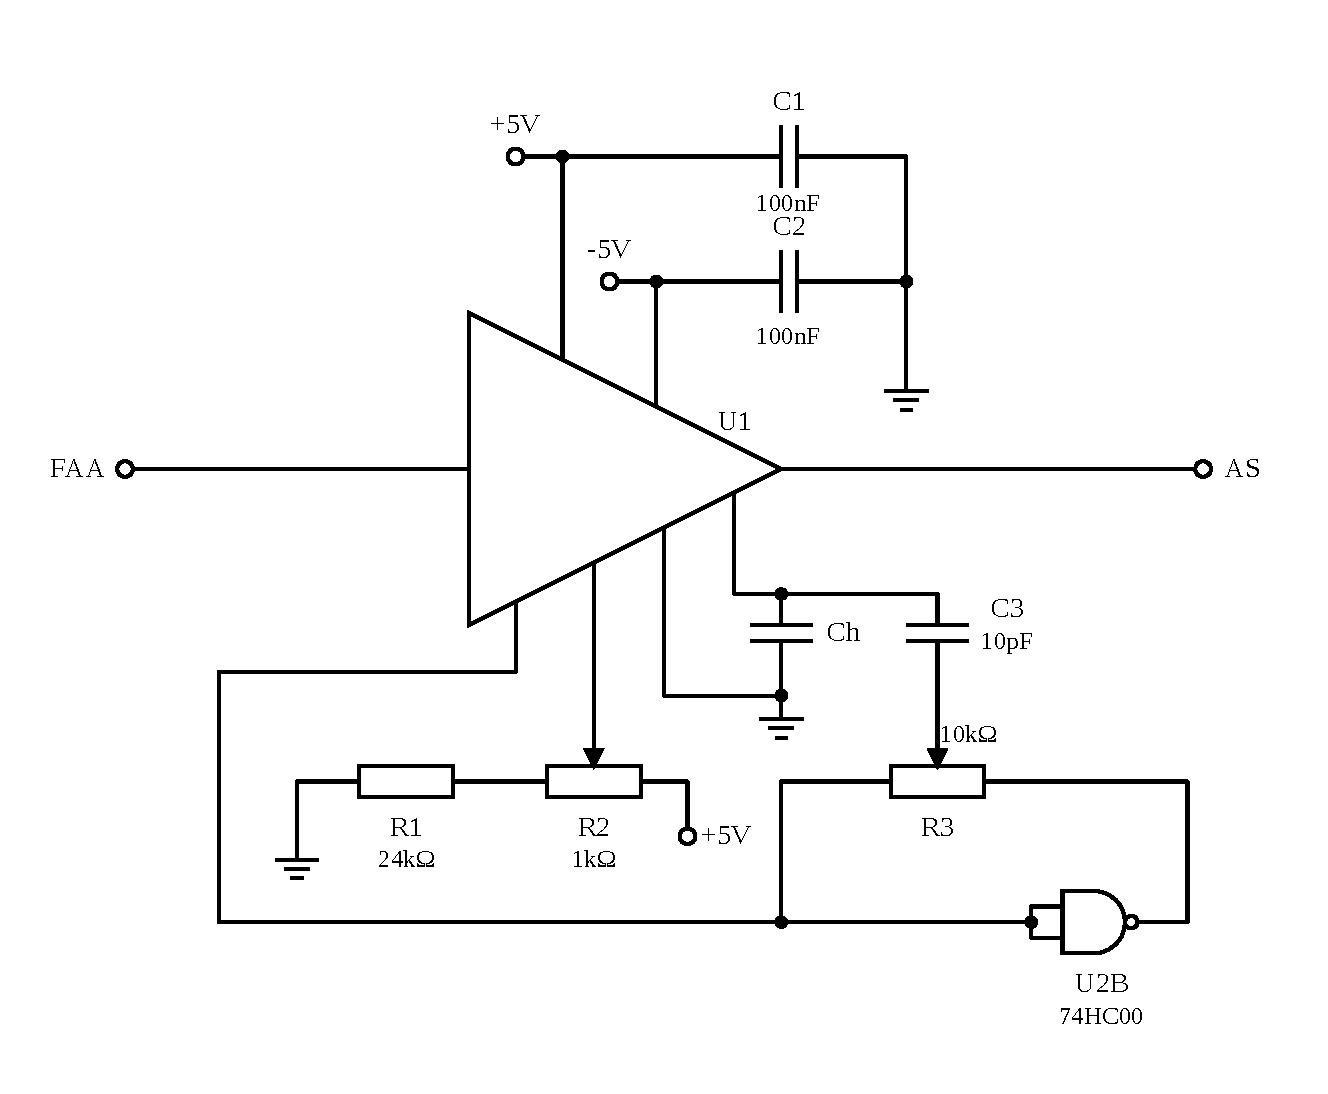
\includegraphics[width = 0.6\textwidth]{Imagenes/4_S&H/S&H_Config.pdf}
	\caption{Conexiones hechas para el integrado LF398}
	\label{fig: filtro}
\end{figure}

\subsection{Circuito Integrado \textit{Sample and Hold} Alternativo}

Como alternativa de alto rendimiento frente al clásico LF398, el estándar de la industria en adquisición de datos suele apuntar a integrados monolíticos de mayor velocidad y precisión, destacándose el \textbf{AD585} (fabricado por Analog Devices). 

A continuación, se presenta un análisis comparativo justificado con los parámetros directos de su respectiva hoja de especificaciones:

\subsubsection*{Análisis de la Alternativa: Analog Devices AD585}

El AD585 es un circuito completo de muestreo y retención diseñado para instrumentación y sistemas de conversión de 10 y 12 bits. Se compone de un amplificador operacional de alta velocidad en serie con un interruptor analógico de fuga ultrabaja y un amplificador integrador de entrada FET.

\begin{itemize}
	\item \textbf{Ventajas frente al LF398:}
	\begin{itemize}
		\item \textbf{Capacitor interno integrado:} A diferencia del LF398, el cual depende exclusivamente de un componente externo, el AD585 incluye su propio capacitor de \textit{hold} de grado de precisión directamente en el silicio (típicamente $100\text{ pF}$). Esto elimina gran parte de los problemas de histéresis y las fugas parásitas en la superficie de la placa (PCB), logrando una tasa de caída (\textit{droop rate}) garantizada y especificada de apenas $1.0\text{ mV/ms}$ como máximo.
		\item \textbf{Error de salto (\textit{Hold Step}) acotado:} En su \textit{datasheet}, el error inducido por la inyección de carga al abrir la llave está especificado a un máximo estricto de $3\text{ mV}$. Al ser holgadamente menor a nuestro margen de error para un conversor de 8 bits ($1 LSB \approx 19.53\text{ mV}$), se puede prescindir de circuitos externos de cancelación dinámica (\textit{AC Zeroing}) complejos, simplificando el ruteo de la placa.
		\item \textbf{Tiempo de adquisición veloz y garantizado:} El fabricante asegura un tiempo máximo de $3.0\text{ }\mu\text{s}$ para que la salida se asiente con una precisión del $\pm 0.01\%$ frente a un escalón de $10\text{V}$. Esto vuelve predecible el diseño temporal y permite frecuencias de muestreo significativamente mayores que las obtenidas con el LF398.
	\end{itemize}
	
	\item \textbf{Desventajas:}
	\begin{itemize}
		\item \textbf{Pérdida de flexibilidad de diseño:} Al contar con el capacitor fijo internamente, el diseñador no tiene la misma libertad que en el LF398 para manipular la relación de compromiso fundamental (Velocidad de \textit{Sample} vs. \textit{Droop Rate} en \textit{Hold}). Aunque el AD585 permite añadir capacitancia externa extra para reducir el \textit{droop}, hacerlo penaliza fuertemente el excelente tiempo de adquisición nativo del chip.
		\item \textbf{Costo comercial:} Dado que es un componente monolítico enfocado en la alta instrumentación y sistemas aeroespaciales, su costo por unidad es notablemente superior al de las familias genéricas.
	\end{itemize}
\end{itemize}